\newcommand{\ee}{\mathrm{e}}
\newcommand{\ii}{\mathrm{i}}
\heading{数学物理方法（上）-第4次作业}

\begin{question}
计算积分 \[
I=\oint_{C} (z-a)^n \dd{z},
\] 其中 \(C\) 为任意可求长简单闭合曲线，\(n \in \mathbb{Z}\).
\begin{solution}
对于 \(n \ge 0\) 的情况，\((z-a)^n\) 在 \(\mathbb{C}\) 上解析，因此由柯西定理可知 \( I=0. \)

对于 \(n < 0\) 的情况，\((z-a)^n\) 在 \(\mathbb{C} \setminus \{a\}\) 上解析，因此若 \(C\) 不包含 \(a\)，则同样由柯西定理 \( I=0. \)

若 \(C\) 包含 \(a\)，可以考察如下回路：

\begin{center}
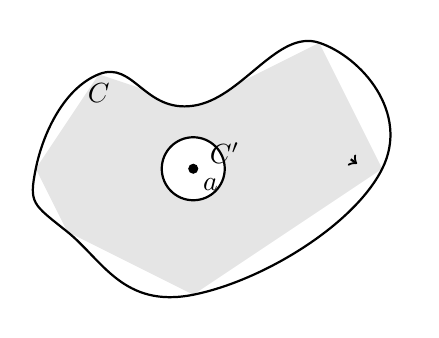
\begin{tikzpicture}[scale=0.8]
  % Fill the region between the outer loop and inner circle
  \begin{scope}
    \clip plot[smooth cycle,tension=0.8] coordinates {
      (3,0) (2,2) (0,1) (-1.5,1.5) (-2.5,0) (-2,-1) (0,-2)
    };
    \fill[gray!20] (3,0) -- (2,2) -- (0,1) -- (-1.5,1.5) -- (-2.5,0) -- (-2,-1) -- (0,-2) -- cycle;
    \fill[white] (0,0) circle (0.5);
  \end{scope}

  % Draw the outer loop
  \draw[thick] plot[smooth cycle,tension=0.8] coordinates {
    (3,0) (2,2) (0,1) (-1.5,1.5) (-2.5,0) (-2,-1) (0,-2)
  };

  % Arrow indicator on the outer loop
  \draw[->,thick] (2.5,0.15) -- (2.6,0.08);

  % Draw the inner circle
  \draw[thick] (0,0) circle (0.5);

  % Point a at center
  \filldraw (0,0) circle (2pt) node[below right] {$a$};

  % Labels
  \node at (0.5,0.25) {$C'$};
  \node at (-1.5,1.2) {$C$};
\end{tikzpicture}
\end{center}

其中 \(C'\) 为以 \(a\) 为圆心，\(r\) 为半径的小圆。函数在灰色区域内是解析的，因此有 \[
I=-\oint_{C'} (z-a)^n \dd{z}=-\int_{0}^{2\pi} [r \ee^{\ii \theta}]^n \dd{}(r \ee^{\ii \theta})=-r^{n+1} \int_{0}^{2\pi} \ii \ee^{\ii(n+1) \theta} \dd{}\theta,
\] 故当 \(n=-1\) 时，有 \[
I=\int_{0}^{2\pi} -\ii \dd{}\theta = -2\pi \ii,
\] 当 \(n \neq -1\) 时，有 \(I=0.\)

综上有：
\begin{center}
\fbox{\begin{minipage}{0.8\linewidth}
\begin{itemize}
    \item 若 \(n\neq -1\)，则 \(\displaystyle \oint_{C} (z-a)^n \dd{z}=0\)
    \item 若 \(n=-1\)，则 \(\displaystyle \oint_{C} (z-a)^n \dd{z}=
    \begin{cases}
    0, & C\text{不包含} a,\\
    -2\pi \ii, & C\text{包含} a
    \end{cases}\)
\end{itemize}
\end{minipage}}
\end{center}
\end{solution}
\end{question}
